\begin{figure}[tbp]
\centering
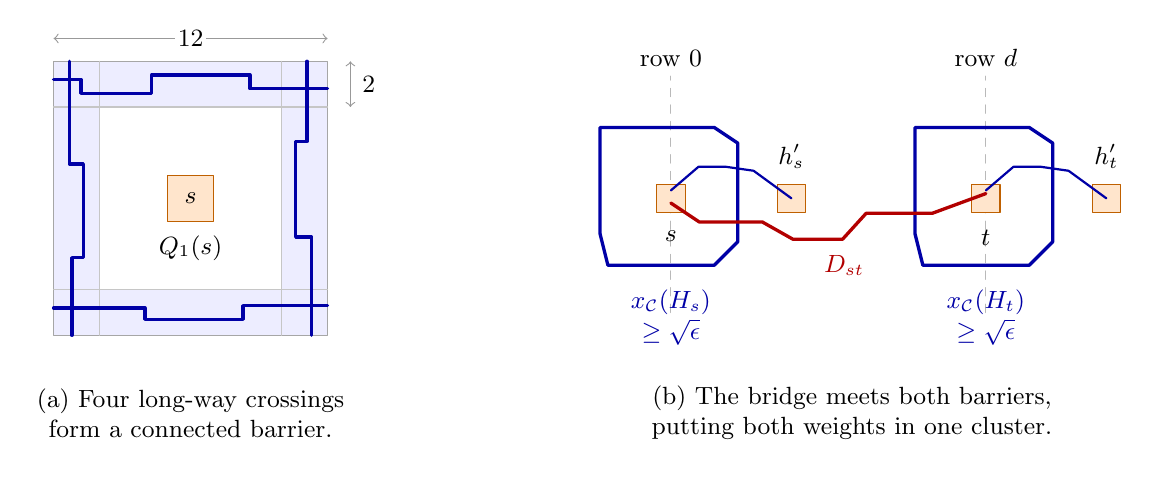
\begin{tikzpicture}[font=\small,line cap=round,line join=round]
 \begin{scope}[x=0.29cm,y=0.29cm]
  \fill[blue!7] (-6,-6) rectangle (6,6);
  \fill[white] (-4,-4) rectangle (4,4);
  \draw[gray!70] (-6,-6) rectangle (6,6);
  \draw[gray!70,dashed] (-4,-4) rectangle (4,4);
  \draw[gray!45] (-6,4)--(6,4) (-6,-4)--(6,-4)
                  (-4,-6)--(-4,6) (4,-6)--(4,6);
  \filldraw[fill=orange!20,draw=orange!75!black]
      (-1,-1) rectangle (1,1);
  \node at (0,0) {$s$};
  \node[anchor=north] at (0,-1.2) {$Q_1(s)$};
  \draw[blue!65!black,very thick]
     (-6,5.2)--(-4.8,5.2)--(-4.8,4.6)--(-1.7,4.6)
       --(-1.7,5.4)--(2.6,5.4)--(2.6,4.8)--(6,4.8);
  \draw[blue!65!black,very thick]
     (5.1,6)--(5.1,2.5)--(4.6,2.5)--(4.6,-1.7)
       --(5.3,-1.7)--(5.3,-6);
  \draw[blue!65!black,very thick]
     (6,-4.7)--(2.3,-4.7)--(2.3,-5.3)--(-2,-5.3)
       --(-2,-4.8)--(-6,-4.8);
  \draw[blue!65!black,very thick]
     (-5.2,-6)--(-5.2,-2.6)--(-4.7,-2.6)--(-4.7,1.5)
       --(-5.3,1.5)--(-5.3,6);
  \draw[<->,gray!80] (-6,7)--(6,7);
  \node[fill=white,inner sep=1pt] at (0,7) {$12$};
  \draw[<->,gray!80] (7,4)--(7,6);
  \node[anchor=west] at (7.1,5) {$2$};
  \node[align=center] at (0,-9.4)
     {(a) Four long-way crossings\\form a connected barrier.};
 \end{scope}
 \begin{scope}[shift={(6.1cm,0cm)},x=1cm,y=1cm]
  \draw[gray!55,dashed] (0,-1.45)--(0,1.55);
  \draw[gray!55,dashed] (4.0,-1.45)--(4.0,1.55);
  \node[above] at (0,1.55) {row $0$};
  \node[above] at (4,1.55) {row $d$};
  \foreach \u in {0,4} {
   \filldraw[fill=orange!20,draw=orange!75!black]
      (\u-0.18,-0.18) rectangle (\u+0.18,0.18);
   \filldraw[fill=orange!20,draw=orange!75!black]
      (\u+1.35,-0.18) rectangle (\u+1.71,0.18);
   \draw[blue!65!black,very thick]
      (\u-0.8,-0.85)--(\u+0.55,-0.85)--(\u+0.85,-0.55)
       --(\u+0.85,0.7)--(\u+0.55,0.9)--(\u-0.9,0.9)
       --(\u-0.9,-0.45)--cycle;
   \draw[blue!65!black,thick]
      (\u,0.1)--(\u+0.35,0.4)--(\u+0.7,0.4)
       --(\u+1.05,0.35)--(\u+1.53,0);
  }
  \draw[red!70!black,very thick]
    (0,-0.06)--(0.36,-0.3)--(1.16,-0.3)--(1.55,-0.52)
      --(2.18,-0.52)--(2.48,-0.19)--(3.32,-0.19)--(4,0.06);
  \node[below=3pt] at (0,-0.18) {$s$};
  \node[below=3pt] at (4,-0.18) {$t$};
  \node[above=2pt] at (1.53,0.18) {$h'_s$};
  \node[above=2pt] at (5.53,0.18) {$h'_t$};
  \node[red!70!black,below] at (2.2,-0.6) {$D_{st}$};
  \node[blue!65!black,below,align=center] at (0,-1.04)
      {$x_{\mathcal C}(H_s)$\\$\ge\sqrt\epsilon$};
  \node[blue!65!black,below,align=center] at (4,-1.04)
      {$x_{\mathcal C}(H_t)$\\$\ge\sqrt\epsilon$};
  \node[align=center] at (2.3,-2.72)
     {(b) The bridge meets both barriers,\\putting both weights in one cluster.};
 \end{scope}
\end{tikzpicture}
\caption{The geometric step in \eqref{vis:bridge}.
In (a), neighboring strip crossings meet in the corner squares.
In (b), on $A_s\cap A_t$, each barrier carries normalized weight
from the tests inside and outside it; any path in $D_{st}$ joins the
two barrier clusters.  Orange squares show test supports.  Panel (b)
is schematic: time runs horizontally and the distance between the
rings is compressed.}
\label{fig:circuits}
\end{figure}
